\subsection{Flow properties}

\begin{proposition}{}{repeat_has_several_incoming_arcs}
  A fragment is a repeat if several link-arcs are incoming to it.
\end{proposition}

\begin{proof}
  Immediate from the fact that an active arc has a flow of value at least \(F\).
\end{proof}

\begin{proposition}{Incoming flows are not multiple of the total flow}{inflow_is_not_multiple_of_total_flow}
  \[
    \exists N = (V, A_\Fragments{} \cup A_\Links{}, s, t, \cov{\Fragments{}}), a \in A_\Links{}, k \in \Naturals{}
    \mid k F < f_a < (k + 1) F
  \]
\end{proposition}

\begin{proof}
  \zcref[S]{fig:inflow_not_multiple_total_flow} illustrates the following proof.

  Let build the network \(N = (V, A_\Fragments{} \cup A_\Links{}, s, t, \cov{\Fragments{}})\) where (the dots mean to complete with the reverse arcs):
  \begin{align*}
    & \Fragments{} = \Set{a, b, c, d} \\
    & \cov{a} = 4 \quad \cov{b} = 8 \quad \cov{c} = 10 \quad \cov{d} = 4 \\
    & A_\Links{} = \Set{
      (s, a_t), (a_h, b_t), (b_h, c_t), (c_h, c_t), (c_h, b_t), (b_h, t), \ldots
    }
  \end{align*}
  The incoming flows maximizing the coverage score are:
  \[
    f_{s a_t} = 4 \quad f_{a_h b_t} = 4 \quad f_{b_h c_t} = 4 \quad f_{c_h c_t} = 6 \quad f_{c_h b_t} = 4 \quad f_{b_h t} = 4
  \] implying a total flow of \(F = 4\).
  In this example, the incoming flow \(f_{c_h c_t} = 6\) is not a multiple of \(F = 4\), and we found an integer \(k = 1\) such that \(k F < f_{c_h c_t} < (k + 1) F\).
\end{proof}

\begin{figure}
  \centering
  \begin{subfigure}[b]{0.45\linewidth}
    \centering
    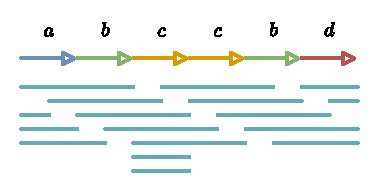
\includegraphics[width=\linewidth]{appendix/method/img/inflow_not_multiple_total_flow-true_sequencing.pdf}
    \caption{True sequencing}\label{subfig:inflow_not_multiple_total_flow-true_sequencing}
  \end{subfigure}
  \hfill
  \begin{subfigure}[b]{0.45\linewidth}
    \centering
    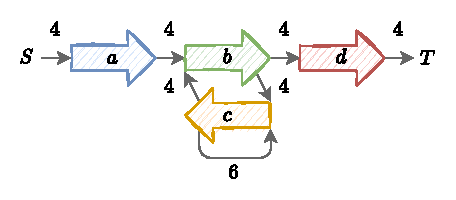
\includegraphics[width=\linewidth]{appendix/method/img/inflow_not_multiple_total_flow-MCF_solution.pdf}
    \caption{MCF solution}\label{subfig:inflow_not_multiple_total_flow-MCF_solution}
  \end{subfigure}
  \figurecaption{Non-uniform sequencing depth can imply incoming flows to not be a multiple of the total flow.}{
    Each coloured arrow is a sequence.
    \Subref{subfig:inflow_not_multiple_total_flow-true_sequencing}
    A genome cut into four regions, where \(b\) and \(c\) are both direct repeats of occurence two.
    The reads are turquoise lines, aligned to the regions.
    Two reads imply an irregular sequencing depth for region \(c\).
    \Subref{subfig:inflow_not_multiple_total_flow-MCF_solution}
    An instance of network associated to \subref{subfig:inflow_not_multiple_total_flow-true_sequencing}.
    The coverage on sequences are \(4\) for \(a\) and \(d\), \(8\) for \(b\), and \(10\) for \(c\).
    The total flow \(F = 4\).
    Incoming flows perfectly equals to the coverage of each sequence.
    The flow on the arc \((c_h, c_t) \in A_\Links{}\) is not a multiple of \(F\).
  }\label{fig:inflow_not_multiple_total_flow}
\end{figure}